\section{Results}

Two sets of data were taken, and are examined here in terms of the accuracy of
their produced models and the possible causes of error in the reconstruction
process. The first set of photographs were taken at Long Ashton Farm outside
Bristol, and the second set were taken at the Avon Gorge in Bristol.

\subsection{Long Ashton}

For this data set, a hexacopter was used to gather a total of 63 aerial images.
The time interval technique was used to take the photos, and the time offset
method used to geotag the resulting photos.

\subsubsection{Without GCPs}
\label{sec:results/long-ashton/no-gcp}

Firstly, the reconstruction was run without the Ground Control Points input, and
without any photographic alignment optimisation. The resulting orthophoto is
shown in Figure \ref{img:long-ashton/no-gcps/orthophoto}, while the DEM is shown
in Figure \ref{img:long-ashton/no-gcps/dem} and the photographic overlap is shown
in Figure \ref{img:long-ashton/no-gcps/overlap}. The produced model is available
to \href{https://sketchfab.com/models/ad8a1d9f8c324eb592a9e4beabc5a51e}{view
interactively online}.

\begin{figure}
    \centering
    \begin{subfigure}[b]{0.3\textwidth}
        \includegraphics[width=\textwidth]{LongAshton/NoGCPs/Orthophoto}
        \caption{The generated orthophoto for the Long Ashton data set, without
        GCPs input.}
        \label{img:long-ashton/no-gcps/orthophoto}
    \end{subfigure}
    \begin{subfigure}[b]{0.3\textwidth}
        \includegraphics[width=\textwidth]{LongAshton/NoGCPs/DEM}
        \caption{The generated DEM for the Long Ashton data set, without GCPs
        input.}
        \label{img:long-ashton/no-gcps/dem}
    \end{subfigure}
    \begin{subfigure}[b]{0.3\textwidth}
        \includegraphics[width=\textwidth]{LongAshton/NoGCPs/Overlap}
        \caption{The calculated photographic overlap achieved in the Long Ashton
        photo dataset.}
        \label{img:long-ashton/no-gcps/overlap}
    \end{subfigure}
    \caption{The data produced by PhotoScan from the Long Ashton aerial imagery,
    without factoring in GCPs.}
    \label{img:long-ashton/no-gcps}
\end{figure}

Clearly, the orthophoto shows that the 63 photos were sufficient to build a
model of the topography of the area. However, the Digital Elevation Model shows
that the photogrammetric reconstruction interpreted the topography as on a
significant tilt head from the car park up to the building. We hypothesise that
this tilt is due to the lack of GCPs to correct for such systematic errors. This
is discussed with reference to the model produced \textit{with} GCPs in Section
\ref{sec:results/long-ashton/wth-gcps} and also with reference to the Avon Gorge
reconstruction in Section \ref{sec:results/avon-gorge}.

Figure \ref{img:long-ashton/no-gcps/overlap} shows that the overlap between the
photos is more than adequate in all the central areas of the model, only
reducing to \textless 9 around the very edges of the area.

\subsubsection{With GCPs}
\label{sec:results/long-ashton/wth-gcps}

The reconstruction was then rerun with a limited number of Ground Control Points
input. These GCPs were taken using distinguishable features from the landscape
and their geolocation found from Google Earth to test the effect they would have
on the resulting model and DEM. The first DEM was taken as the centre of a pond,
the second the corner of a fence and the third was a cross marked in with white
tape, whose location was approximated by referencing nearby features on Google
Maps. While this is not sufficiently accurate for a true georeference, it
suffices to demonstrate that the tilt is removed from the final model once the
GCPs are introduced.

\begin{figure}
    \centering
    \begin{subfigure}[b]{0.45\textwidth}
        \includegraphics[width=\textwidth]{LongAshton/WithGCPs/Orthophoto}
        \caption{The generated orthophoto for the Long Ashton data set, with 3
        GCPs input.}
        \label{img:long-ashton/with-gcps/orthophoto}
    \end{subfigure}
    \begin{subfigure}[b]{0.45\textwidth}
        \includegraphics[width=\textwidth]{LongAshton/WithGCPs/DEM}
        \caption{The generated DEM for the Long Ashton data set, with 3 GCPs
        input.}
        \label{img:long-ashton/with-gcps/dem}
    \end{subfigure}
    \begin{subfigure}[b]{0.45\textwidth}
        \includegraphics[width=\textwidth]{LongAshton/WithGCPs/Overlap}
        \caption{The calculated photographic overlap achieved in the Long Ashton
        photo dataset with 3 GCPs.}
        \label{img:long-ashton/with-gcps/overlap}
    \end{subfigure}
    \begin{subfigure}[b]{0.45\textwidth}
        \includegraphics[width=\textwidth]{LongAshton/WithGCPs/GCPs}
        \caption{The locations of the placed GCPs.}
        \label{img:long-ashton/with-gcps/gcps}
    \end{subfigure}
    \caption{The data produced by PhotoScan from the Long Ashton aerial imagery,
    with 3 GCPs input.}
    \label{img:long-ashton/with-gcps}
\end{figure}

Figure \ref{img:long-ashton/with-gcps/dem} shows the DEM with these 3 GCPs
introduced into the photogrammetric alignment process. Clearly, the model is no
longer considering on a slope, as it was in Figure
\ref{img:long-ashton/no-gcps/dem}. However, the previously vertical faces are
now tilted themselves, meaning that the wall of the warehouse is not vertically
up, but a tilted slope up to the roof. We argue that this is an artefact of the
small number of GCPs used trying to georeference the model. If the minimum
number of 10 GCPs or more were used, then the software would correctly
georeference the model and the sloped walls would be corrected. Section
\ref{sec:results/avon-gorge/no-gcps} and \ref{sec:results/avon-gorge/with-gcps}
discusses this further with reference to the Avon Gorge photo set, which
contained more than the required number of GCPs.

The data generated by PhotoScan, displayed in Table \ref{tab:long-ashton},
further illustrates the inefficacy of georeferencing with geotagged photos
alone. Not only does the final model appear slanted, but the flying altitude is
incorrectly taken to be \SI{4.9}{m}. Even with only 3 GCPs, this altitude error
is corrected when the GCPs are used to georeference the model as well as the
geotagged photos. This difference in calculated flying altitude also explains
the better ground and DEM resolution for the model reconstructed without GCPs as
opposed to the model reconstructed with the GCPs; the factor by which the GCP
ground and DEM resolution is better is approximately equal to the factor by
which the GCP model flying altitude is higher, taking the slight difference in
error into account. Having a higher flying altitude means each pixel corresponds
to a larger distance.

The errors for both models are approximately equal at $\approx$ \SI{1}{pix},
with a slightly higher error for the model with GCPs. This number
represents the root means square reprojection error calculated over all features
points detected on the photo. Thus, a possible source of the error is that
without the GCPs, the software in unaware of the systematic error demonstrated
by the sloped DEM. When the GCPs are introduced, the software realises that the
systematic error is there, and the value of the reprojection error is increased
accordingly. Even though the GCP georeferenced model has a slightly larger
error, it still corresponds to a very small distance of \SI{0.155}{mm}. This
value is too small to be a realistic value, indicating that the GCPs have not
sufficiently corrected the model to its true value for the error present in the
model to be recognised and reported by PhotoScan. This is supported by the
comparison in Section \ref{sec:results/avon-gorge/with-gcps}.

\begin{table}
    \begin{tabular}{| l | c | c |}
        \hline
        & \textbf{Without GCPs} & \textbf{With GCPs} \\
        \hline
        \textbf{Flying Altitude} (m)       & 4.88261     & 37.1183    \\
        \textbf{Ground Resolution} (m/pix) & 0.000940159 & 0.00622731 \\
        \textbf{Error} (pix)               & 0.971366    & 1.37699    \\
        \textbf{DEM Resolution} (m/pix)    & 0.00376064  & 0.0249093  \\
        \hline
    \end{tabular}
    \caption{The data generated by PhotoScan for the Long Ashton models, with
    and without GCPs.}
    \label{tab:long-ashton}
\end{table}

\subsection{Avon Gorge}
\label{sec:results/avon-gorge}

This model was reconstructed from two passes of 87 and 61 photos. As before, the
time interval with time offset techniques were used for taking photos and
geotagging the photos, respectively. The photos were taken by attaching the
camera to the quadcopter and tilting it by hand to attain horizontally oriented
photographs of the cliff face that is the Avon-Gorge. The purpose of this was to
give useful photos equivalent to aerial photogrammetry before the quadcopter was
ready to fly.

\subsubsection{First Pass Versus Second Pass}
\label{sec:results/avon-gorge/passes}

The first pass was taken facing the gorge horizontally on, thereby fully
representing an equivalent to aerial photogrammetry. The second pass was at an
oblique angle, facing upwards to capture the top of the gorge. As expected, the
second pass at an oblique angle produced less accurate results than the first
pass a zenithal angle to the cliff face. This is shown visually in Figures
\ref{img:avon-gorge/pass-1} and \ref{img:avon-gorge/pass-2}. In particular where
the oblique angle causes the camera to be unable to see the top of the cliff and
where the cliff meets the sky, the model is erroneous. For the former the model
produces clear spikes in the model, jutting from the face of the cliff. For the
latter, the software includes the sky as an extension of the cliff. Masking the
sky out, as described in Section \ref{sec:methods/masking}, removes the latter
problem to a limited extent, but the former remains, as shown in Figure
\ref{img:avon-gorge/pass-2/masked}.

\begin{figure}
    \centering
    \begin{subfigure}[b]{0.45\textwidth}
        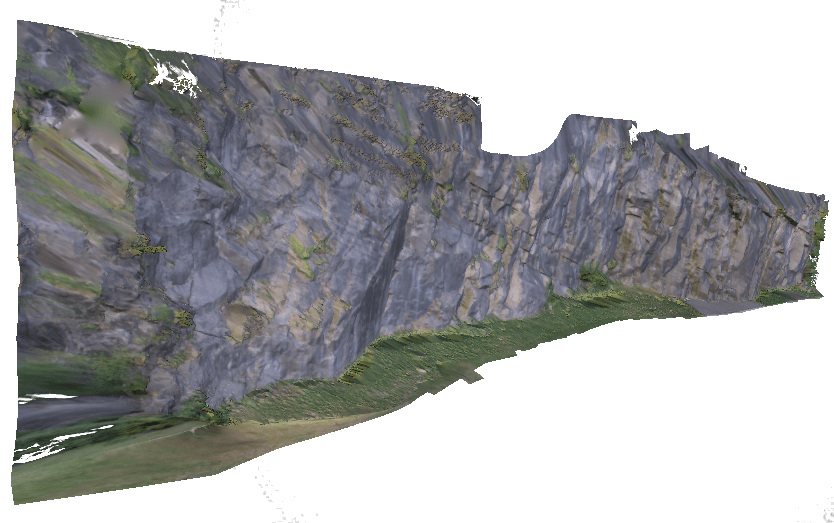
\includegraphics[width=\textwidth]{AvonGorge/Pass1}
        \caption{The model produced using only the first pass of photos at the
        zenithal angle.}
        \label{img:avon-gorge/pass-1}
    \end{subfigure}
    \begin{subfigure}[b]{0.45\textwidth}
        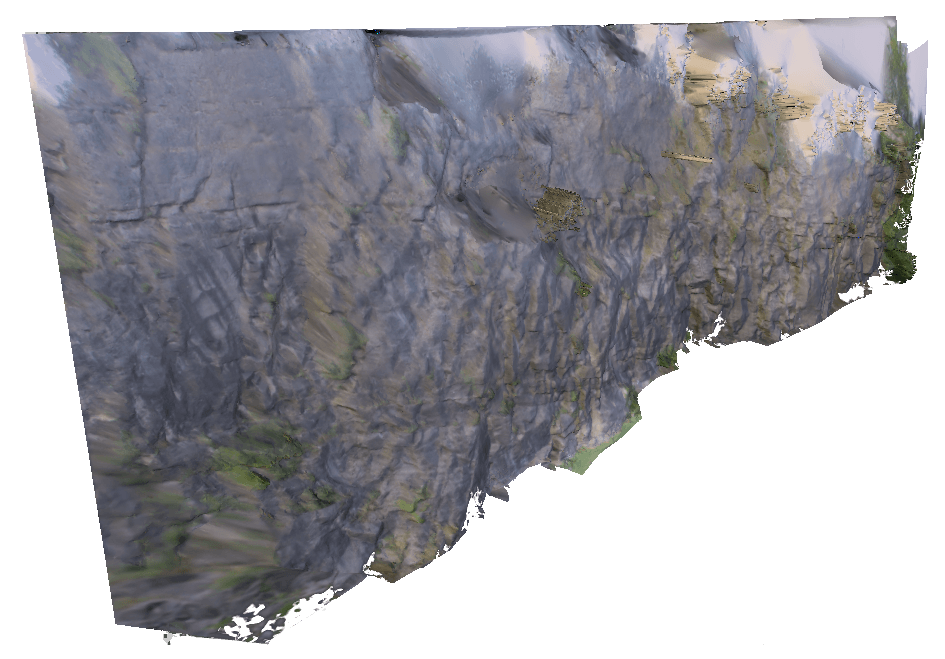
\includegraphics[width=\textwidth]{AvonGorge/Pass2}
        \caption{The model produced using only the second pass of photos at the
        oblique angle.}
        \label{img:avon-gorge/pass-2}
    \end{subfigure}
    \begin{subfigure}[b]{0.9\textwidth}
        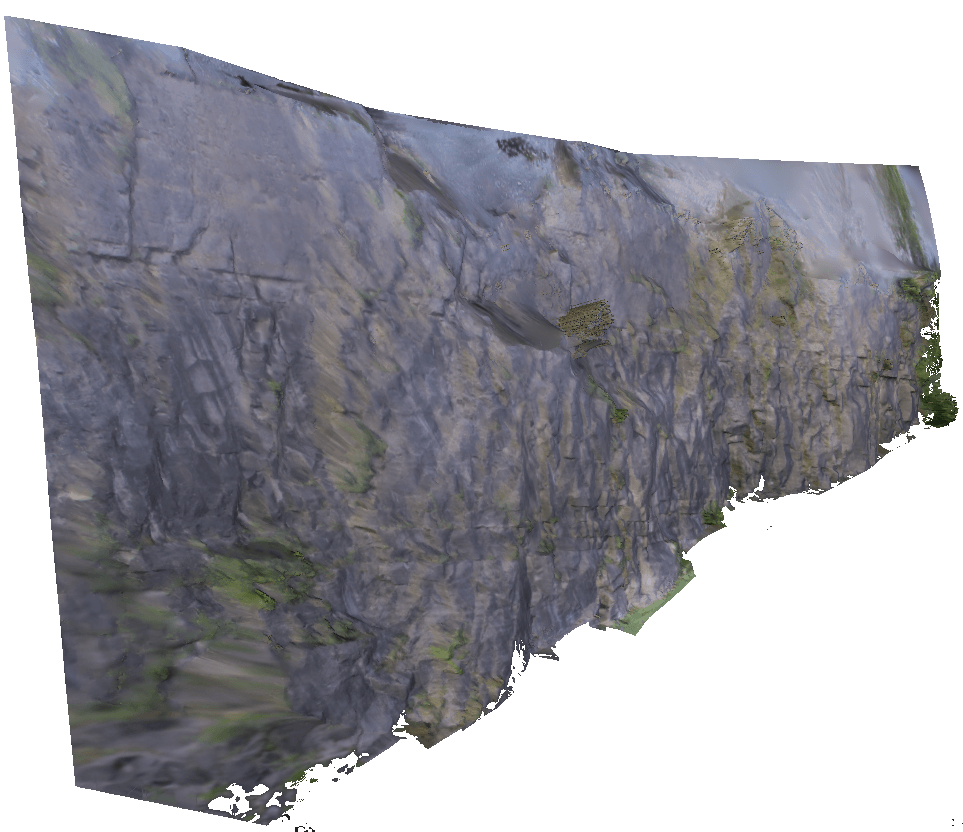
\includegraphics[width=\textwidth]{AvonGorge/Pass2Masked}
        \caption{The model produced using only the second pass of photos,
        masking out the sky.}
        \label{img:avon-gorge/pass-2/masked}
    \end{subfigure}
    \caption{A visual comparison of the relative error induced in the models
    produced in the first and second passes, at zenithal and oblique angles
    respectively.}
    \label{img:avon-gorge/passes}
\end{figure}

\subsubsection{Without GCPs}
\label{sec:results/avon-gorge/no-gcps}

When the first pass is taken with no GCPs input, there are several important
emergent features to note.

Firstly, as Figure \ref{img:avon-gorge/no-gcps/cameras} shows, the calculated
locations of the cameras was very inaccurate, with some errors extending beyond
the model. This is because the geolocation of the photos from the on-board UAV
GPS is simply not accurate enough to be the only method of georeferencing; the
GCPs are also needed in addition to the geotagged photo locations.

Secondly, as Figure \ref{img:avon-gorge/no-gcps/dem} shows, the reconstruction
has also incorrectly interpreted the landscape as being on a tilt, with the
north of the gorge (top of the image) appearing higher than the south of the
gorge (bottom of the image). The systematic sloping that these reconstructions
seem to exhibit is a strange if irrelevant phenomenon (so long as a sufficient
number of GCPs are provided), possibly caused by the camera being tilted as it
is attached to the UAVs.

\begin{figure}
    \centering
    \begin{subfigure}[b]{0.24\textwidth}
        \includegraphics[width=\textwidth]{AvonGorge/NoGCPs/Orthophoto}
        \caption{The generated orthophoto for the Avon Gorge data set, no
        GCPs input.}
        \label{img:avon-gorge/no-gcps/orthophoto}
    \end{subfigure}
    \begin{subfigure}[b]{0.24\textwidth}
        \includegraphics[width=\textwidth]{AvonGorge/NoGCPs/DEM}
        \caption{The generated DEM for the Avon Gorge data set, no GCPs input.}
        \label{img:avon-gorge/no-gcps/dem}
    \end{subfigure}
    \begin{subfigure}[b]{0.24\textwidth}
        \includegraphics[width=\textwidth]{AvonGorge/NoGCPs/Overlap}
        \caption{The calculated photographic overlap achieved in the Avon Gorge
        photo dataset no GCPs.}
        \label{img:avon-gorge/no-gcps/overlap}
    \end{subfigure}
    \begin{subfigure}[b]{0.24\textwidth}
        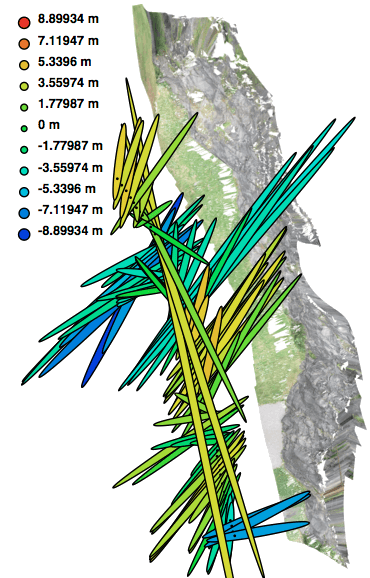
\includegraphics[width=\textwidth]{AvonGorge/NoGCPs/Cameras}
        \caption{The calculated positions of the cameras, along with the errors
        involved in these calculations, representation as ellipses.}
        \label{img:avon-gorge/no-gcps/cameras}
    \end{subfigure}
    \caption{The data produced by PhotoScan from the Avon Gorge horizontal
    imagery, no GCPs input.}
    \label{img:avon-gorge/no-gcps}
\end{figure}

\subsubsection{With GCPs}
\label{sec:results/avon-gorge/with-gcps}

Once the GCPs are input, there are several important effects.

The photographic overlap of the gorge increases, with only the very corners
having less than 9 overlapped photos covering it. With more accurate
georeferencing, the software recognises the photos as taken more spread apart,
and thus with better coverage of the corners of the model.

The tilt present in Figure \ref{img:avon-gorge/no-gcps/dem} disappears, as shown
in Figure \ref{img:avon-gorge/with-gcps/dem}. The produced model now correctly
identifies the bottom of the gorge as level. This indicates that the slopes
present in the Avon Gorge and Long Ashton models are merely artefacts of the
lack of GCPs, which, when the sufficient number of GCPs are introduced,
disappears.

\begin{figure}
    \centering
    \begin{subfigure}[b]{0.45\textwidth}
        \includegraphics[width=\textwidth]{AvonGorge/WithGCPs/Orthophoto}
        \caption{The generated orthophoto for the Avon Gorge data set, with 14
        GCPs input.}
        \label{img:avon-gorge/with-gcps/orthophoto}
    \end{subfigure}
    \begin{subfigure}[b]{0.45\textwidth}
        \includegraphics[width=\textwidth]{AvonGorge/WithGCPs/DEM}
        \caption{The generated DEM for the Avon Gorge data set, with 14 GCPs
        input.}
        \label{img:avon-gorge/with-gcps/dem}
    \end{subfigure}
    \begin{subfigure}[b]{0.45\textwidth}
        \includegraphics[width=\textwidth]{AvonGorge/WithGCPs/Overlap}
        \caption{The calculated photographic overlap achieved in the Avon Gorge
        photo dataset with 14 GCPs.}
        \label{img:avon-gorge/with-gcps/overlap}
    \end{subfigure}
    \begin{subfigure}[b]{0.45\textwidth}
        \includegraphics[width=\textwidth]{AvonGorge/WithGCPs/GCPs}
        \caption{The positions of the input GCPs.}
        \label{img:avon-gorge/with-gcps/gcps}
    \end{subfigure}
    \caption{The data produced by PhotoScan from the Avon Gorge horizontal
    imagery, with 14 GCPs input.}
    \label{img:avon-gorge/with-gcps}
\end{figure}

The data produced by PhotoScan is shown in Table \ref{tab:avon-gorge}. As in
Table \ref{tab:long-ashton}, the flying altitude is increased significantly for
the GCP georeferenced model, although in this context the flying altitude has
less meaning owing to the fact that the photographs of the gorge were taken
horizontally. As before, the ground resolution is better, again due to the
different value of the flying altitude inferred from the software.

The difference in reprojection error is more pronounced here, which could be
explained by the higher number of GCPs; with the model fully accurately
georeferenced, the errors in the reprojection are fully realised and reported by
PhotoScan, meaning that the reported error is higher. It's important to note
that, as before, even the higher value of the error for the GCP georeferenced
model, which corresponds to a value in meters of \SI{1.24}{cm}, is well within
an acceptable range. The fact that this value is also realistic indicates that
the previously unrealistically small error in Section
\ref{sec:results/long-ashton/with-gcps} was indeed a result of not having enough
GCPs to properly georeference the model, thereby resulting in PhotoScan not
fully recognising the error present in the model.

\begin{table}
    \begin{tabular}{| l | c | c |}
        \hline
        & \textbf{Without GCPs} & \textbf{With GCPs} \\
        \hline
        \textbf{Flying Altitude} (m)       & 16.5655    & 51.5781    \\
        \textbf{Ground Resolution} (m/pix) & 0.00339199 & 0.00260205 \\
        \textbf{Error} (pix)               & 1.02017    & 4.76105    \\
        \textbf{DEM Resolution} (m/pix)    & 0.013568   & 0.0692152  \\
        \hline
    \end{tabular}
    \caption{The PhotoScan generated data for the Avon Gorge models, with and
    without GCPs.}
    \label{tab:avon-gorge}
\end{table}
